
\AtBeginSection[]
{
    \small\begin{frame}
        \frametitle{目录}
        \tableofcontents[
            sectionstyle=show/shaded,
            subsectionstyle=show/show/hide,
            subsubsectionstyle=show/show/show/hide
        ]
    \end{frame}
}
\maketitle
\begin{frame}
    \frametitle{目录}
    \tableofcontents[hideallsubsections]
    \small 笔记见 \url{https://ernestdong.github.io/posts/machine_learning_in_erm/},

    \small 源代码见 \url{https://github.com/ErnestDong/ml-in-erm}

    \small 强烈推荐 \href{https://www.youtube.com/watch?v=Ye018rCVvOo&list=PLJV_el3uVTsMhtt7_Y6sgTHGHp1Vb2P2J}{李宏毅机器学习}
    \small 与 \href{https://zh-v2.d2l.ai/}{李沐动手深度学习}
\end{frame}

\section{前言}
\subsection{机器学习概述}
\begin{frame}
    \frametitle{何谓“机器学习”}
    \begin{columns}
        \column{0.6\linewidth}
        \includegraphics[width=.9\textwidth]{/Users/dcy/Code/ernest/static/images/xkcd/1838.png}
        \column{0.35\linewidth}
        真实世界中集合的关系可以用函数抽象,机器学习其实就是让机器去拟合这个函数/概率密度函数。我将尝试用经典的几个算法来给大家举例机器是如何拟合的。

        \begin{definition}
            机器学习是一门人工智能的科学,该领域的主要研究对象是人工智能,特别是如何在经验学习中改善具体算法的性能。
        \end{definition}
    \end{columns}
\end{frame}
\subsection{机器学习的分类}
\begin{frame}
    \frametitle{机器学习的分类}
    \begin{columns}
        \column{0.6\linewidth}
        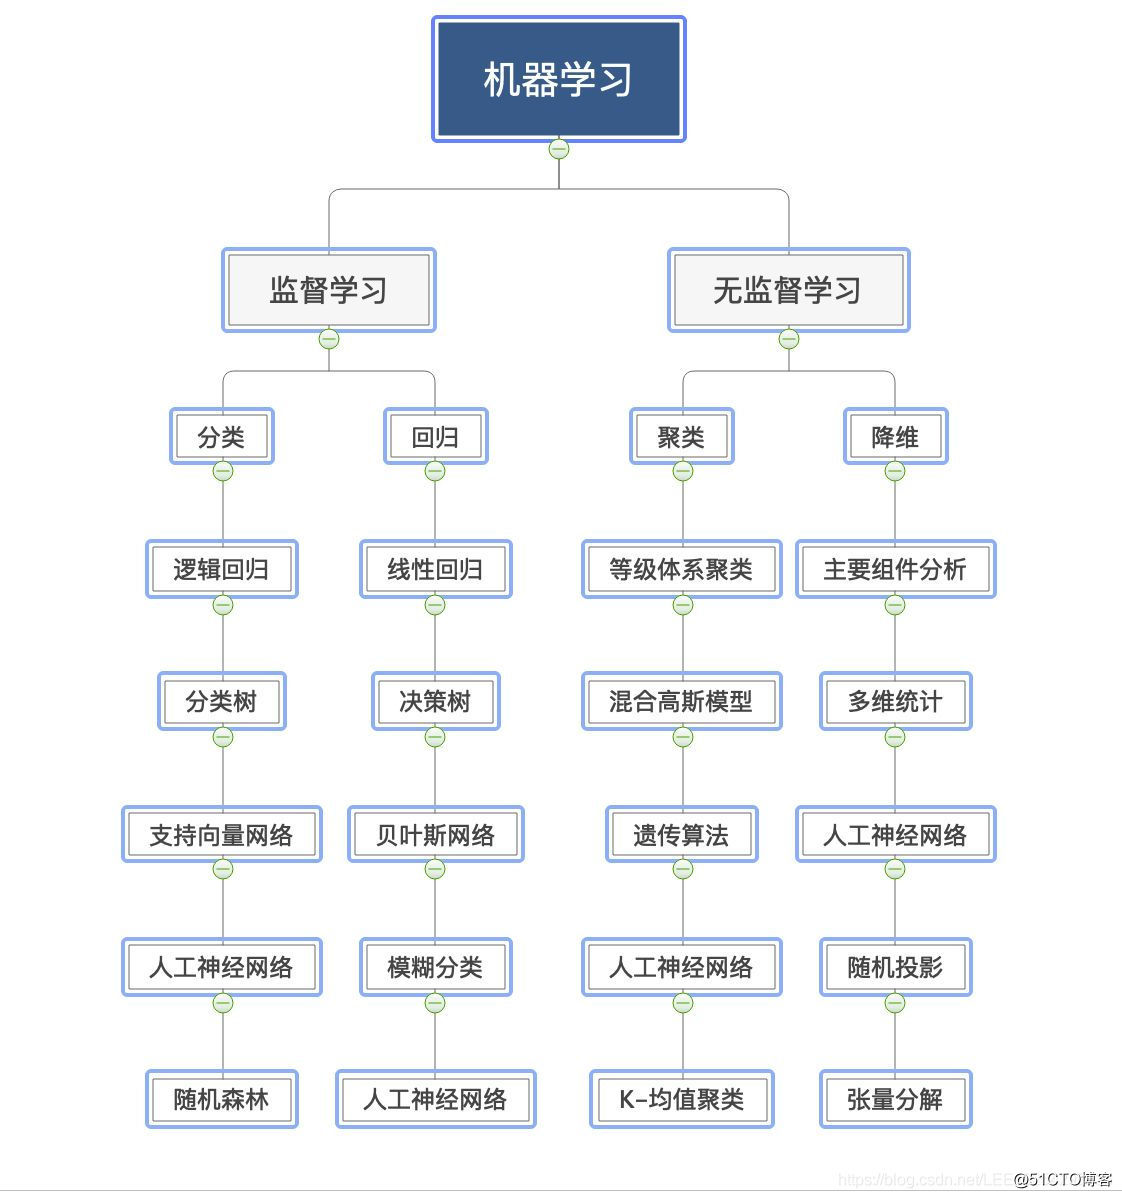
\includegraphics[width=.9\textwidth]{../lib/机器学习.jpeg}
        \column{0.35\linewidth}
        机器学习深究的话,需要学习很多数学和计算机知识。
        但是工业界将常用的机器学习算法封装地很好(如pytorch, scikit-learn),几行代码就可以实现一个简单的模型。我们就采用“硬 Train 一发”的方式了解一下经典的算法。

        本文主要参考了\textcite{scikit-learn}的文档,在编码过程中阅读文档是有帮助的。
    \end{columns}
\end{frame}
\section{机器学习预测信用评级}
\subsection{数据预处理}
\begin{frame}
    \frametitle{数据来源}
    数据来自 \href{https://www.kaggle.com/datasets/agewerc/corporate-credit-rating}{kaggle}。
    涵盖了 2029 家美国上市公司信用评级的历史数据。数据除了公司基本信息外,还包括了30个财务特征:

    \begin{enumerate}
        \item 流动性指标: currentRatio, quickRatio, cashRatio, daysOfSalesOutstanding
        \item 盈利能力: grossProfitMargin, operatingProfitMargin, pretaxProfitMargin, netProfitMargin, effectiveTaxRate, returnOnAssets, returnOnEquity, returnOnCapitalEmployed
        \item 负债比率: debtRatio, debtEquityRatio
        \item 营运表现: assetTurnover, fixedasset
        \item 现金流指标: operatingCashFlowPerShare, freeCashFlowPerShare, cashPerShare, operatingCashFlowSalesRatio, freeCashFlowOperatingCashFlowRatio
    \end{enumerate}
\end{frame}
\begin{frame}[fragile]
    \frametitle{数据简单处理}
    评级分布如图\ref{rating}所示。
    我们会合并 C/CC/CCC 的评级,选取 3/4 作为训练集,1/4 作为测试集。
    \begin{figure}
        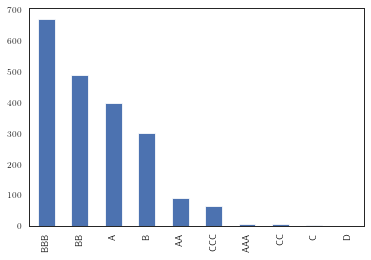
\includegraphics[width=0.6\linewidth]{../lib/rating.png}
        \label{rating}
        \caption{评级分布}
    \end{figure}
\end{frame}
\begin{frame}[fragile]
    \frametitle{数据简单处理}
    \begin{minted}{python}
import pandas as pd
import matplotlib.pyplot as plt
import seaborn as sns
df = pd.read_csv("./corporate_rating.csv", encoding="utf-8")
Y = df["Rating"].replace({"CCC": "C", "CC": "C"})
df["Date"] = df["Date"].apply(lambda x: x.split("/")[-1])
dummies = ["Rating Agency Name", "Sector", "Date"]
X = df[[i for i in df.columns if df[i].dtype != "object"]]
X = pd.concat([X]+[pd.get_dummies(df[i], drop_first=True)
    for i in dummies]),
    axis=1)
Xtrain, Xtest, Ytrain, Ytest = train_test_split(
    X, Y, test_size=0.25, random_state=42
)
\end{minted}
\end{frame}
\begin{frame}
    \frametitle{评价机器学习效果的指标}
    对于二分类问题,一个样本真实情况可能是 True/False,对应预测可能是 Positive/Negative。
    \begin{center}
        \begin{tabular}{lll}
                     & True & False \\
            Positive & TP   & FP    \\
            Negative & TN   & FN    \\
        \end{tabular}
    \end{center}
    \begin{definition}{精确率、召回率、F1}
        \begin{eqnarray}
            precision & = & TP / (TP + FP) \nonumber\\
            recall & = & TP / (TP + FN) \nonumber\\
            F1 & = & \frac{precision\cdot recall}{precision+recall}\nonumber
        \end{eqnarray}
    \end{definition}
    分别为 预测阳性中真实为正的概率、样本中的正例有多少被预测正确、以及二者的调和平均。
\end{frame}

\begin{frame}[fragile]
    \frametitle{评价机器学习效果的指标}
    除此之外,我们再来比较一下“相关系数”,看一看预测差异是否很大。
    \begin{minted}{python}
def get_score(Xtest, Ytrue, model):
    Ypred = model(Xtest)
    avg = "weighted"
    rating_map = {i: ord(i[0]) * 100 - len(i)
                    for i in Y.unique()}
    return {
        "precision":
            precision_score(Ytrue, Ypred, average=avg),
        "recall": recall_score(Ytrue, Ypred, average=avg),
        "f1": f1_score(Ytrue, Ypred, average=avg),
        "\(R^2\)": pearsonr(
            [rating_map[i] for i in Ypred],
            [rating_map[i] for i in Ytest]
        )[0],
    }
\end{minted}
\end{frame}
\begin{frame}
    \frametitle{完全随机的情况}
    如果我们训练的分类器完全无效,那么结果如表\ref{random}所示。
    \begin{table}
        \caption{随机的情况}
        \begin{tabular}{ll}
            precision & 0.2364 \\
            recall    & 0.1254 \\
            f1        & 0.1544 \\
            \(R^2\)   & 0.0089 \\
        \end{tabular}
        \label{random}
    \end{table}
\end{frame}
